\chapter{A Flurry in Stocks}

Some days after this meeting, Albert de Morcerf visited the Count of
Monte Cristo at his house in the Champs-Élysées, which had already
assumed that palace-like appearance which the count’s princely fortune
enabled him to give even to his most temporary residences. He came to
renew the thanks of Madame Danglars which had been already conveyed to
the count through the medium of a letter, signed “Baronne Danglars,
\textit{née} Hermine de Servieux.”

Albert was accompanied by Lucien Debray, who, joining in his friend’s
conversation, added some passing compliments, the source of which the
count’s talent for finesse easily enabled him to guess. He was
convinced that Lucien’s visit was due to a double feeling of curiosity,
the larger half of which sentiment emanated from the Rue de la Chaussée
d’Antin. In short, Madame Danglars, not being able personally to
examine in detail the domestic economy and household arrangements of a
man who gave away horses worth 30,000 francs and who went to the opera
with a Greek slave wearing diamonds to the amount of a million of
money, had deputed those eyes, by which she was accustomed to see, to
give her a faithful account of the mode of life of this
incomprehensible person. But the count did not appear to suspect that
there could be the slightest connection between Lucien’s visit and the
curiosity of the baroness.

“You are in constant communication with the Baron Danglars?” the count
inquired of Albert de Morcerf.

“Yes, count, you know what I told you?”

“All remains the same, then, in that quarter?”

“It is more than ever a settled thing,” said Lucien,—and, considering
that this remark was all that he was at that time called upon to make,
he adjusted the glass to his eye, and biting the top of his gold headed
cane, began to make the tour of the apartment, examining the arms and
the pictures.

“Ah,” said Monte Cristo “I did not expect that the affair would be so
promptly concluded.”

“Oh, things take their course without our assistance. While we are
forgetting them, they are falling into their appointed order; and when,
again, our attention is directed to them, we are surprised at the
progress they have made towards the proposed end. My father and M.
Danglars served together in Spain, my father in the army and M.
Danglars in the commissariat department. It was there that my father,
ruined by the revolution, and M. Danglars, who never had possessed any
patrimony, both laid the foundations of their different fortunes.”

“Yes,” said Monte Cristo “I think M. Danglars mentioned that in a visit
which I paid him; and,” continued he, casting a side-glance at Lucien,
who was turning over the leaves of an album, “Mademoiselle Eugénie is
pretty—I think I remember that to be her name.”

“Very pretty, or rather, very beautiful,” replied Albert, “but of that
style of beauty which I do not appreciate; I am an ungrateful fellow.”

“You speak as if you were already her husband.”

“Ah,” returned Albert, in his turn looking around to see what Lucien
was doing.

“Really,” said Monte Cristo, lowering his voice, “you do not appear to
me to be very enthusiastic on the subject of this marriage.”

“Mademoiselle Danglars is too rich for me,” replied Morcerf, “and that
frightens me.”

“Bah,” exclaimed Monte Cristo, “that’s a fine reason to give. Are you
not rich yourself?”

“My father’s income is about 50,000 francs per annum; and he will give
me, perhaps, ten or twelve thousand when I marry.”

“That, perhaps, might not be considered a large sum, in Paris
especially,” said the count; “but everything does not depend on wealth,
and it is a fine thing to have a good name, and to occupy a high
station in society. Your name is celebrated, your position magnificent;
and then the Comte de Morcerf is a soldier, and it is pleasing to see
the integrity of a Bayard united to the poverty of a Duguesclin;
disinterestedness is the brightest ray in which a noble sword can
shine. As for me, I consider the union with Mademoiselle Danglars a
most suitable one; she will enrich you, and you will ennoble her.”

Albert shook his head, and looked thoughtful.

“There is still something else,” said he.

“I confess,” observed Monte Cristo, “that I have some difficulty in
comprehending your objection to a young lady who is both rich and
beautiful.”

“Oh,” said Morcerf, “this repugnance, if repugnance it may be called,
is not all on my side.”

“Whence can it arise, then? for you told me your father desired the
marriage.”

“It is my mother who dissents; she has a clear and penetrating
judgment, and does not smile on the proposed union. I cannot account
for it, but she seems to entertain some prejudice against the
Danglars.”

\begin{figure}[ht]
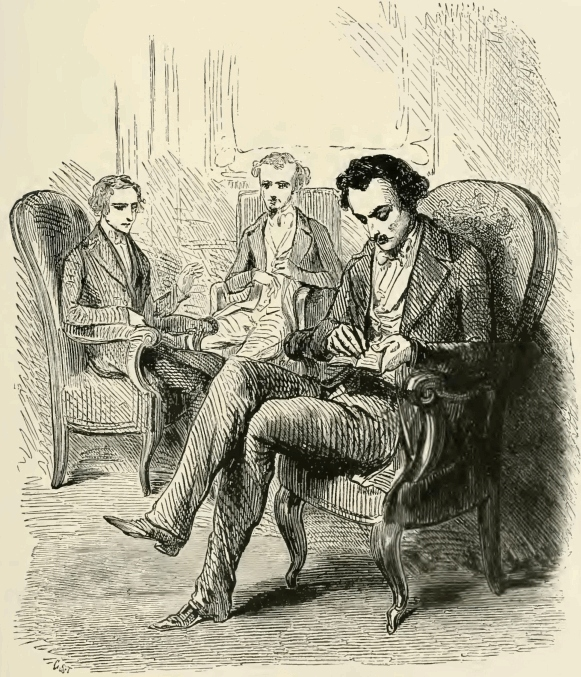
\includegraphics[width=\textwidth]{30107m.jpg}
\end{figure}

“Ah,” said the count, in a somewhat forced tone, “that may be easily
explained; the Comtesse de Morcerf, who is aristocracy and refinement
itself, does not relish the idea of being allied by your marriage with
one of ignoble birth; that is natural enough.”

“I do not know if that is her reason,” said Albert, “but one thing I do
know, that if this marriage be consummated, it will render her quite
miserable. There was to have been a meeting six weeks ago in order to
talk over and settle the affair; but I had such a sudden attack of
indisposition——”

“Real?” interrupted the count, smiling.

“Oh, real enough, from anxiety doubtless,—at any rate they postponed
the matter for two months. There is no hurry, you know. I am not yet
twenty-one, and Eugénie is only seventeen; but the two months expire
next week. It must be done. My dear count, you cannot imagine how my
mind is harassed. How happy you are in being exempt from all this!”

“Well, and why should not you be free, too? What prevents you from
being so?”

“Oh, it will be too great a disappointment to my father if I do not
marry Mademoiselle Danglars.”

“Marry her then,” said the count, with a significant shrug of the
shoulders.

“Yes,” replied Morcerf, “but that will plunge my mother into positive
grief.”

“Then do not marry her,” said the count.

“Well, I shall see. I will try and think over what is the best thing to
be done; you will give me your advice, will you not, and if possible
extricate me from my unpleasant position? I think, rather than give
pain to my dear mother, I would run the risk of offending the count.”

Monte Cristo turned away; he seemed moved by this last remark.

“Ah,” said he to Debray, who had thrown himself into an easy-chair at
the farthest extremity of the salon, and who held a pencil in his right
hand and an account book in his left, “what are you doing there? Are
you making a sketch after Poussin?”

“Oh, no,” was the tranquil response; “I am too fond of art to attempt
anything of that sort. I am doing a little sum in arithmetic.”

“In arithmetic?”

“Yes; I am calculating—by the way, Morcerf, that indirectly concerns
you—I am calculating what the house of Danglars must have gained by the
last rise in Haiti bonds; from 206 they have risen to 409 in three
days, and the prudent banker had purchased at 206; therefore he must
have made 300,000 livres.”

“That is not his biggest scoop,” said Morcerf; “did he not make a
million in Spaniards this last year?”

“My dear fellow,” said Lucien, “here is the Count of Monte Cristo, who
will say to you, as the Italians do,—

\hspace{1cm}“‘Denaro e santità,

\hspace{1cm}Metà della metà.’\footnote[9]{‘Money and sanctity, Each in a moiety.’}


“When they tell me such things, I only shrug my shoulders and say
nothing.”

“But you were speaking of Haitians?” said Monte Cristo.

“Ah, Haitians,—that is quite another thing! Haitians are the \textit{écarté}
of French stock-jobbing. We may like bouillotte, delight in whist, be
enraptured with boston, and yet grow tired of them all; but we always
come back to \textit{écarté}—it is not only a game, it is a \textit{hors-d’œuvre}! M.
Danglars sold yesterday at 405, and pockets 300,000 francs. Had he but
waited till today, the price would have fallen to 205, and instead of
gaining 300,000 francs, he would have lost 20 or 25,000.”

“And what has caused the sudden fall from 409 to 206?” asked Monte
Cristo. “I am profoundly ignorant of all these stock-jobbing
intrigues.”

“Because,” said Albert, laughing, “one piece of news follows another,
and there is often great dissimilarity between them.”

“Ah,” said the count, “I see that M. Danglars is accustomed to play at
gaining or losing 300,000 francs in a day; he must be enormously rich.”

“It is not he who plays!” exclaimed Lucien; “it is Madame Danglars; she
is indeed daring.”

“But you who are a reasonable being, Lucien, and who knows how little
dependence is to be placed on the news, since you are at the
fountain-head, surely you ought to prevent it,” said Morcerf, with a
smile.

“How can I, if her husband fails in controlling her?” asked Lucien;
“you know the character of the baroness—no one has any influence with
her, and she does precisely what she pleases.”

“Ah, if I were in your place——” said Albert.

“Well?”

“I would reform her; it would be rendering a service to her future
son-in-law.”

“How would you set about it?”

“Ah, that would be easy enough—I would give her a lesson.”

“A lesson?”

“Yes. Your position as secretary to the minister renders your authority
great on the subject of political news; you never open your mouth but
the stockbrokers immediately stenograph your words. Cause her to lose a
hundred thousand francs, and that would teach her prudence.”

“I do not understand,” stammered Lucien.

“It is very clear, notwithstanding,” replied the young man, with an
artlessness wholly free from affectation; “tell her some fine morning
an unheard-of piece of intelligence—some telegraphic despatch, of which
you alone are in possession; for instance, that Henri IV. was seen
yesterday at Gabrielle’s. That would boom the market; she will buy
heavily, and she will certainly lose when Beauchamp announces the
following day, in his gazette, ‘The report circulated by some usually
well-informed persons that the king was seen yesterday at Gabrielle’s
house, is totally without foundation. We can positively assert that his
majesty did not quit the Pont-Neuf.’”

Lucien half smiled. Monte Cristo, although apparently indifferent, had
not lost one word of this conversation, and his penetrating eye had
even read a hidden secret in the embarrassed manner of the secretary.
This embarrassment had completely escaped Albert, but it caused Lucien
to shorten his visit; he was evidently ill at ease. The count, in
taking leave of him, said something in a low voice, to which he
answered, “Willingly, count; I accept.” The count returned to young
Morcerf.

“Do you not think, on reflection,” said he to him, “that you have done
wrong in thus speaking of your mother-in-law in the presence of M.
Debray?”

“My dear count,” said Morcerf, “I beg of you not to apply that title so
prematurely.”

“Now, speaking without any exaggeration, is your mother really so very
much averse to this marriage?”

“So much so that the baroness very rarely comes to the house, and my
mother, has not, I think, visited Madame Danglars twice in her whole
life.”

“Then,” said the count, “I am emboldened to speak openly to you. M.
Danglars is my banker; M. de Villefort has overwhelmed me with
politeness in return for a service which a casual piece of good fortune
enabled me to render him. I predict from all this an avalanche of
dinners and routs. Now, in order not to presume on this, and also to be
beforehand with them, I have, if agreeable to you, thought of inviting
M. and Madame Danglars, and M. and Madame de Villefort, to my
country-house at Auteuil. If I were to invite you and the Count and
Countess of Morcerf to this dinner, I should give it the appearance of
being a matrimonial meeting, or at least Madame de Morcerf would look
upon the affair in that light, especially if Baron Danglars did me the
honor to bring his daughter. In that case your mother would hold me in
aversion, and I do not at all wish that; on the contrary, I desire to
stand high in her esteem.”

“Indeed, count,” said Morcerf, “I thank you sincerely for having used
so much candor towards me, and I gratefully accept the exclusion which
you propose. You say you desire my mother’s good opinion; I assure you
it is already yours to a very unusual extent.”

\begin{figure}[ht]
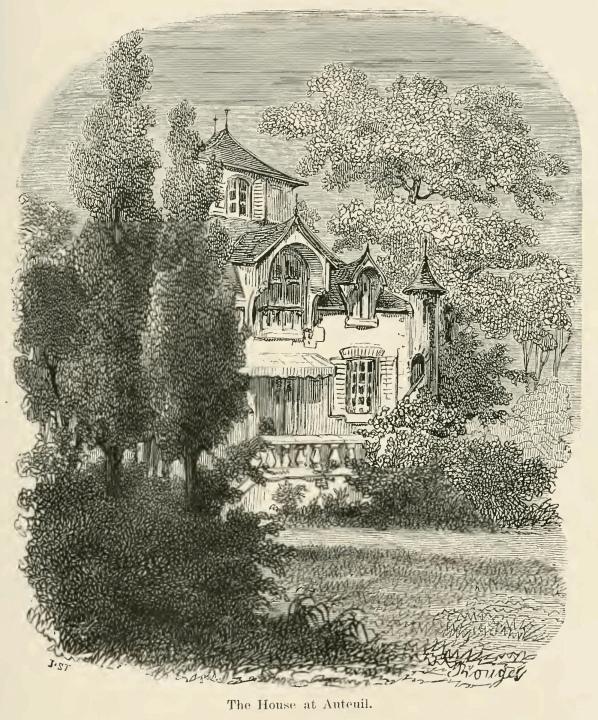
\includegraphics[width=\textwidth]{30111m.jpg}
\end{figure}

“Do you think so?” said Monte Cristo, with interest.

“Oh, I am sure of it; we talked of you an hour after you left us the
other day. But to return to what we were saying. If my mother could
know of this attention on your part—and I will venture to tell her—I am
sure that she will be most grateful to you; it is true that my father
will be equally angry.” The count laughed.

“Well,” said he to Morcerf, “but I think your father will not be the
only angry one; M. and Madame Danglars will think me a very
ill-mannered person. They know that I am intimate with you—that you
are, in fact; one of the oldest of my Parisian acquaintances—and they
will not find you at my house; they will certainly ask me why I did not
invite you. Be sure to provide yourself with some previous engagement
which shall have a semblance of probability, and communicate the fact
to me by a line in writing. You know that with bankers nothing but a
written document will be valid.”

“I will do better than that,” said Albert; “my mother is wishing to go
to the sea-side—what day is fixed for your dinner?”

“Saturday.”

“This is Tuesday—well, tomorrow evening we leave, and the day after we
shall be at Tréport. Really, count, you have a delightful way of
setting people at their ease.”

“Indeed, you give me more credit than I deserve; I only wish to do what
will be agreeable to you, that is all.”

“When shall you send your invitations?”

“This very day.”

“Well, I will immediately call on M. Danglars, and tell him that my
mother and myself must leave Paris tomorrow. I have not seen you,
consequently I know nothing of your dinner.”

“How foolish you are! Have you forgotten that M. Debray has just seen
you at my house?”

“Ah, true.”

“Fix it this way. I have seen you, and invited you without any
ceremony, when you instantly answered that it would be impossible for
you to accept, as you were going to Tréport.”

“Well, then, that is settled; but you will come and call on my mother
before tomorrow?”

“Before tomorrow?—that will be a difficult matter to arrange, besides,
I shall just be in the way of all the preparations for departure.”

“Well, you can do better. You were only a charming man before, but, if
you accede to my proposal, you will be adorable.”

“What must I do to attain such sublimity?”

“You are today free as air—come and dine with me; we shall be a small
party—only yourself, my mother, and I. You have scarcely seen my
mother; you shall have an opportunity of observing her more closely.
She is a remarkable woman, and I only regret that there does not exist
another like her, about twenty years younger; in that case, I assure
you, there would very soon be a Countess and Viscountess of Morcerf. As
to my father, you will not see him; he is officially engaged, and dines
with the chief referendary. We will talk over our travels; and you, who
have seen the whole world, will relate your adventures—you shall tell
us the history of the beautiful Greek who was with you the other night
at the Opera, and whom you call your slave, and yet treat like a
princess. We will talk Italian and Spanish. Come, accept my invitation,
and my mother will thank you.”

“A thousand thanks,” said the count, “your invitation is most gracious,
and I regret exceedingly that it is not in my power to accept it. I am
not so much at liberty as you suppose; on the contrary, I have a most
important engagement.”

“Ah, take care, you were teaching me just now how, in case of an
invitation to dinner, one might creditably make an excuse. I require
the proof of a pre-engagement. I am not a banker, like M. Danglars, but
I am quite as incredulous as he is.”

“I am going to give you a proof,” replied the count, and he rang the
bell.

“Humph,” said Morcerf, “this is the second time you have refused to
dine with my mother; it is evident that you wish to avoid her.”

Monte Cristo started. “Oh, you do not mean that,” said he; “besides,
here comes the confirmation of my assertion.”

Baptistin entered, and remained standing at the door.

“I had no previous knowledge of your visit, had I?”

“Indeed, you are such an extraordinary person, that I would not answer
for it.”

“At all events, I could not guess that you would invite me to dinner.”

“Probably not.”

“Well, listen, Baptistin, what did I tell you this morning when I
called you into my laboratory?”

“To close the door against visitors as soon as the clock struck five,”
replied the valet.

“What then?”

“Ah, my dear count,” said Albert.

“No, no, I wish to do away with that mysterious reputation that you
have given me, my dear viscount; it is tiresome to be always acting
Manfred. I wish my life to be free and open. Go on, Baptistin.”

“Then to admit no one except Major Bartolomeo Cavalcanti and his son.”

“You hear—Major Bartolomeo Cavalcanti—a man who ranks amongst the most
ancient nobility of Italy, whose name Dante has celebrated in the tenth
canto of \textit{The Inferno}, you remember it, do you not? Then there is his
son, Andrea, a charming young man, about your own age, viscount,
bearing the same title as yourself, and who is making his entry into
the Parisian world, aided by his father’s millions. The major will
bring his son with him this evening, the \textit{contino}, as we say in Italy;
he confides him to my care. If he proves himself worthy of it, I will
do what I can to advance his interests. You will assist me in the work,
will you not?”

“Most undoubtedly. This Major Cavalcanti is an old friend of yours,
then?”

“By no means. He is a perfect nobleman, very polite, modest, and
agreeable, such as may be found constantly in Italy, descendants of
very ancient families. I have met him several times at Florence,
Bologna and Lucca, and he has now communicated to me the fact of his
arrival in Paris. The acquaintances one makes in travelling have a sort
of claim on one; they everywhere expect to receive the same attention
which you once paid them by chance, as though the civilities of a
passing hour were likely to awaken any lasting interest in favor of the
man in whose society you may happen to be thrown in the course of your
journey. This good Major Cavalcanti is come to take a second view of
Paris, which he only saw in passing through in the time of the Empire,
when he was on his way to Moscow. I shall give him a good dinner, he
will confide his son to my care, I will promise to watch over him, I
shall let him follow in whatever path his folly may lead him, and then
I shall have done my part.”

“Certainly; I see you are a model Mentor,” said Albert “Good-bye, we
shall return on Sunday. By the way, I have received news of Franz.”

“Have you? Is he still amusing himself in Italy?”

“I believe so; however, he regrets your absence extremely. He says you
were the sun of Rome, and that without you all appears dark and cloudy;
I do not know if he does not even go so far as to say that it rains.”

“His opinion of me is altered for the better, then?”

“No, he still persists in looking upon you as the most incomprehensible
and mysterious of beings.”

“He is a charming young man,” said Monte Cristo “and I felt a lively
interest in him the very first evening of my introduction, when I met
him in search of a supper, and prevailed upon him to accept a portion
of mine. He is, I think, the son of General d’Épinay?”

“He is.”

“The same who was so shamefully assassinated in 1815?”

“By the Bonapartists.”

“Yes. Really I like him extremely; is there not also a matrimonial
engagement contemplated for him?”

“Yes, he is to marry Mademoiselle de Villefort.”

“Indeed?”

\begin{figure}[ht]
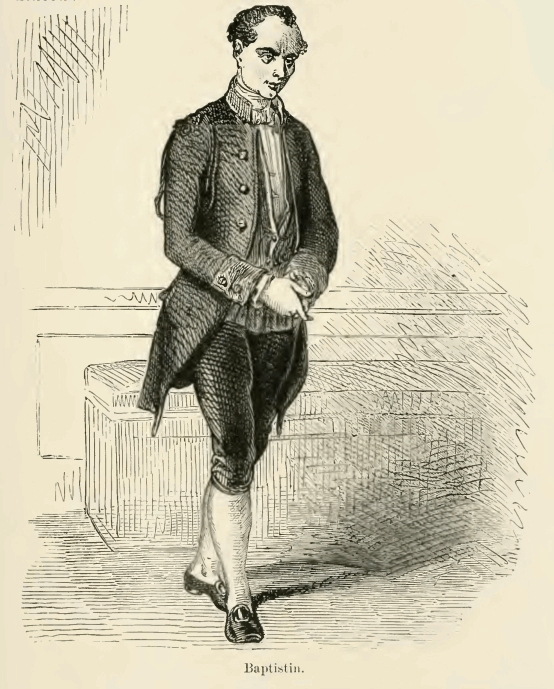
\includegraphics[width=\textwidth]{30115m.jpg}
\end{figure}

“And you know I am to marry Mademoiselle Danglars,” said Albert,
laughing.

“You smile.”

“Yes.”

“Why do you do so?”

“I smile because there appears to me to be about as much inclination
for the consummation of the engagement in question as there is for my
own. But really, my dear count, we are talking as much of women as they
do of us; it is unpardonable.”

Albert rose.

“Are you going?”

“Really, that is a good idea!—two hours have I been boring you to death
with my company, and then you, with the greatest politeness, ask me if
I am going. Indeed, count, you are the most polished man in the world.
And your servants, too, how very well behaved they are; there is quite
a style about them. Monsieur Baptistin especially; I could never get
such a man as that. My servants seem to imitate those you sometimes see
in a play, who, because they have only a word or two to say, aquit
themselves in the most awkward manner possible. Therefore, if you part
with M. Baptistin, give me the refusal of him.”

“By all means.”

“That is not all; give my compliments to your illustrious Luccanese,
Cavalcante of the Cavalcanti; and if by any chance he should be wishing
to establish his son, find him a wife very rich, very noble on her
mother’s side at least, and a baroness in right of her father, I will
help you in the search.”

“Ah, ha; you will do as much as that, will you?”

“Yes.”

“Well, really, nothing is certain in this world.”

“Oh, count, what a service you might render me! I should like you a
hundred times better if, by your intervention, I could manage to remain
a bachelor, even were it only for ten years.”

“Nothing is impossible,” gravely replied Monte Cristo; and taking leave
of Albert, he returned into the house, and struck the gong three times.
Bertuccio appeared.

“Monsieur Bertuccio, you understand that I intend entertaining company
on Saturday at Auteuil.” Bertuccio slightly started. “I shall require
your services to see that all be properly arranged. It is a beautiful
house, or at all events may be made so.”

“There must be a good deal done before it can deserve that title, your
excellency, for the tapestried hangings are very old.”

“Let them all be taken away and changed, then, with the exception of
the sleeping-chamber which is hung with red damask; you will leave that
exactly as it is.” Bertuccio bowed. “You will not touch the garden
either; as to the yard, you may do what you please with it; I should
prefer that being altered beyond all recognition.”

“I will do everything in my power to carry out your wishes, your
excellency. I should be glad, however, to receive your excellency’s
commands concerning the dinner.”

“Really, my dear M. Bertuccio,” said the count, “since you have been in
Paris, you have become quite nervous, and apparently out of your
element; you no longer seem to understand me.”

“But surely your excellency will be so good as to inform me whom you
are expecting to receive?”

“I do not yet know myself, neither is it necessary that you should do
so. ‘Lucullus dines with Lucullus,’ that is quite sufficient.”

Bertuccio bowed, and left the room.
